\chapter {История unix}
\section {Рождение}
UNIX родился в 1969 году, как учебный проект, на малоиспользуемой PDP-8 ???? что стояла в углу.
Первоначально UNIX был написан на ассемблере, но уже в 1971 году был переписан на C, с целью облегчения понимания и портируемости. В результате стало возможным портирование UNIX на другие системы с минимальными модификациями (только ассемблерные вставки, без изменения C-кода).
\section {Развитие}
\subsection {Коммерческий UNIX}
UNIX стал популярен в результате одного исторического решения: AT\&T стала раздавать UNIX университетам, вместе с исходным кодом (для возможности модификации под свои нужды). Это, а так же то, что UNIX в тот момент был достаточно прост (порядка 10000 строк кода), привело к тому, что учебные курсы стали ориентироваться на UNIX, и изучать его устройство. Как следствие это привело к распространению популярности UNIX-а за пределы университетской среды вместе с выпускниками.
\subsection {Свободные альтернативы}
Следующей исторической вехой стоит назвать создание Ричардом Столлманом FSF (Free Software Foundation) в 1984??? году. 

В 1991 году Линус Торвальдс ???
%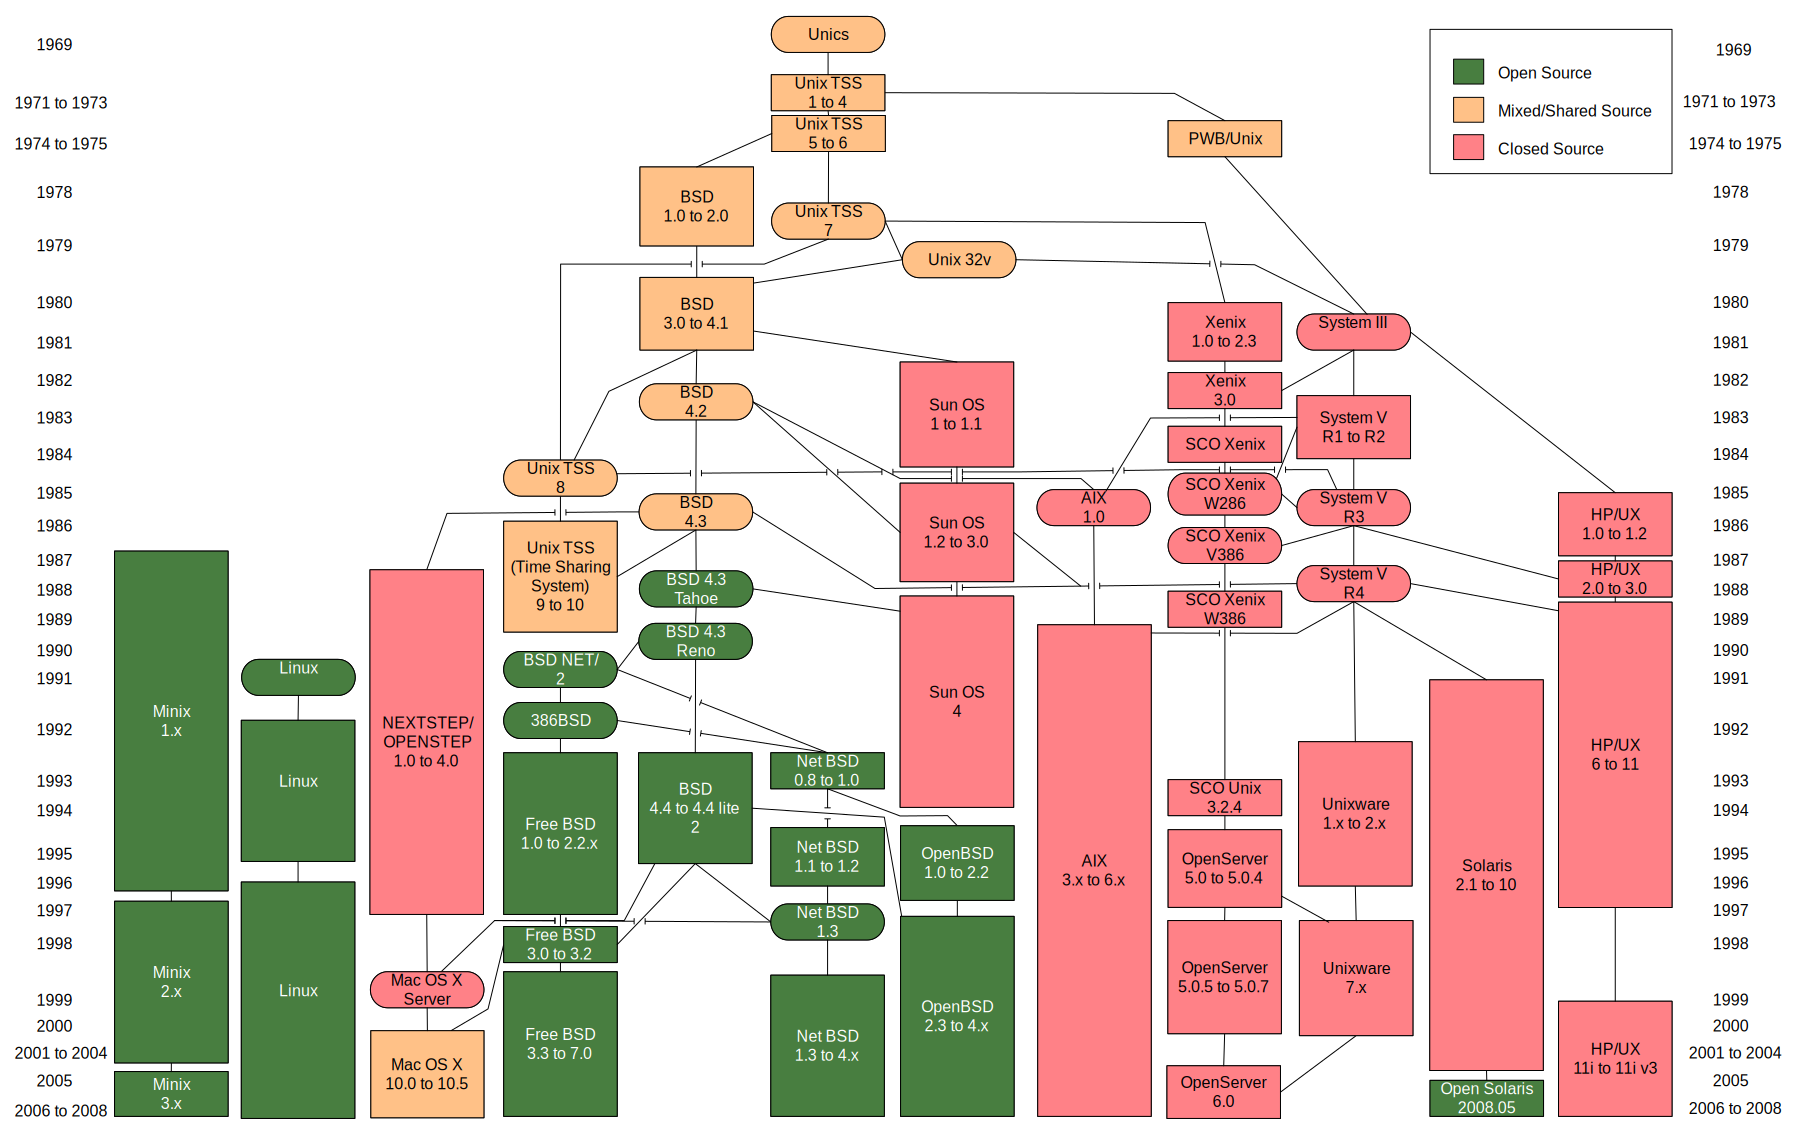
\includegraphics{unix_history}
\section {Стандарты}
\subsection {Single UNIX Specification}
Single UNIX Specification это общее название стандартов, которым должна соответствовать операционная система, чтобы называться «Unix». SUS разрабатывается и поддерживается Austin Group на основе предыдущих разработок IEEE и The Open Group.
\subsection {Степени совместимости и версии стандарта}
Существуют несколько степеней совместимости, нумерующихся по году:
\begin{enumerate}
\item UNIX 93
\item UNIX 95
\item UNIX 98 (удовлетворяет SUS версии 2 ( частичная совместимость )
\item UNIX 03 (удовлетворяет SUS версии 3 ( полная совместимость )
\end{enumerate}
\subsection{Зарегистрированные UNIX-подобные системы}

AIX
    AIX 5L V5.2 с обновлениями, AIX 5L V5.3 и AIX 6.1 совместимы с UNIX 03. AIX 5L V5.2 совместима с UNIX 98.

HP-UX
    HP-UX 11i V3 Release B.11.31 совместима с UNIX 03. Предыдущие версии совместимы с UNIX 95.

IRIX
    IRIX 6.5.28 совместима с UNIX 95.

Mac OS X
    Mac OS X 10.5 «Leopard» и Mac OS X Server 10.5 «Leopard Server» на процессорах Intel совместимы с UNIX 03.

SCO
    UnixWare 7.1.3 совместима с UNIX 95. SCO OpenServer 5 совместима с UNIX 93.

Solaris
    Solaris 10 совместима с UNIX 03 на системах SPARC, 32-/64-битных системах x86 и SPARC64 (Fujitsu PRIMEPOWER). Solaris 8 и 9 совместимы с UNIX 98 на тех же платформах за исключением 64-битных x86. Solaris 2.5.1 была совместима с UNIX 95 на платформе PReP PowerPC в 1996, но продукт был отменён до начала массовых продаж.

Tru64
    Tru64 UNIX V5.1A и далее совместимы с UNIX 98.

z/OS
    IBM z/OS до 1.9 совместима с UNIX 95.

Поставщики Unix-подобных систем, таких как BSD, OpenSolaris и Linux обычно не сертифицируют свои дистрибутивы из-за высокой цены на сертификацию и высокой скорости изменений в этих системах. Схожий стандарт LSB, используемый некоторыми ОС GNU/Linux, опирается на некоторые части SUS.
\section{POSIX}
POSIX
POSIX (англ. Portable Operating System Interface for Unix — Переносимый интерфейс операционных систем Unix) — набор стандартов, описывающих интерфейсы между операционной системой и прикладной программой. Стандарт создан для обеспечения совместимости различных UNIX-подобных операционных систем и переносимости прикладных программ на уровне исходного кода, но может быть использован и для не-Unix систем. Серия стандартов POSIX была разработана комитетом 1003 IEEE. Международная организация по стандартизации (ISO) совместно c Международной электротехнической комиссией (IEC) приняли данный стандарт (POSIX) под названием ISO/IEC 9945.

Название «POSIX» было предложено Ричардом Столлманом. Введение в POSIX.1 гласит: «Ожидается произношение „поз-икс“ как „позитив“, а не „по-сикс“. Произношение опубликовано в целях обнародования стандартного способа ссылки на стандартный интерфейс операционной системы». «POSIX» является зарегистрированным товарным знаком IEEE.[1]

    * 1 Задачи
    * 2 Состав
    * 3 Версии
    * 4 POSIX-совместимые ОС
          o 4.1 Полностью POSIX-совместимые
          o 4.2 По большей части POSIX-совместимые
                + 4.2.1 POSIX для Windows
    * 5 Примечания
    * 6 Литература
    * 7 См. также
    * 8 Ссылки
\subsection{Задачи}
\begin{enumerate}
\item содействие облегчению переноса кода прикладных программ на иные платформы
\item определению и унификация интерфейсов заранее при проектировании, а не в процессе их реализации
\item сохранить по возможности и учитывать все главные, созданные ранее и используемые прикладные программы; ?????
\item определение необходимого минимума интерфейсов прикладных программ, для ускорения создания, одобрения и утверждения документов
\item развитие стандартов в направлении обеспечения коммуникационных сетей, распределенной обработки данных и защиты информации
\item рекомендовать ограничивать использование бинарного (объектного) кода для приложений в простых системах. ?????
\end{enumerate}
\subsection{Состав}
Стандарт состоит из четырёх основных разделов:

\begin{itemize}
\item Основные определения (Base definitions) — список основных определений и соглашений, используемых в спецификациях, и список заголовочных файлов языка Си, которые должны быть предоставлены соответствующей стандарту системой.
\item Оболочка и утилиты (Shell and utilities) — описание утилит и командной оболочки sh, стандарты регулярных выражений.
\item Системные интерфейсы (System interfaces) — список системных вызовов языка Си.
\item Обоснование (Rationale) — объяснение принципов, используемых в стандарте.
\end{itemize}
Помимо основного стандарта (POSIX.1), cуществуют расширения: POSIX.1b и POSIX.1c. Первое из них относится к расширениям реального времени, второе к threads или потоковому выполнению.

POSIX-совместимые ОС

В зависимости от степени совместимости со стандартами, ОС могут быть полностью или частично совместимы с POSIX. Сертифицированные продукты могут быть найдены на сайте IEEE.
Полностью POSIX-совместимые

Полностью соответствующие одной из версий стандарта POSIX: Android OS, A/UX, BSD/OS, HP-UX, IBM AIX, INTEGRITY, IRIX, LynxOS, Mac OS X, Apple iOS, Minix, MPE/iX, OpenSolaris, OpenVMS, QNX, RTEMS, Solaris, UnixWare, velOSity, VxWorks

По большей части POSIX-совместимые

Официально не сертифицированные как POSIX-совместимые, но соответствующие по большей части.
\begin{itemize}
 \item BeOS
 \item FreeBSD
 \item Linux (большинство дистрибутивов — см. LSB)
 \item NetBSD
 \item Nucleus RTOS
 \item OpenBSD
 \item RTEMS
 \item Sanos
 \item SkyOS
 \item Syllable
 \item VSTa
 \item Symbian OS (при помощи PIPS)
\end{itemize}
\subsection{POSIX для Windows}
\begin{itemize}
\item Cygwin — обеспечивает частичное соответствие POSIX для некоторых продуктов Microsoft Windows.
\item Microsoft POSIX subsystem, необязательная подсистема Windows.
\item Microsoft Windows Services for UNIX — обеспечивает полное соответствие POSIX для некоторых продуктов Microsoft Windows. Операционные системы на базе Windows NT до Windows 2000 имели POSIX уровень встроенный в ОС, и UNIX Services for Windows предоставляло UNIX-подобное окружение. Для Windows XP, Windows Services for UNIX должны быть установлены для POSIX совместимости. UNIX подсистема встроена в Enterprise и Ultimate редакции Windows Vista, и не могут быть добавлены в другие редакции.
\item UWIN от ATnT Research обеспечивает POSIX поверх Win32 API.
\end{itemize}
\section{LSB}
Linux Standard Base, LSB — совместный проект нескольких дистрибутивов Linux при организации Linux Foundation, целью которого является стандартизация внутренней структуры операционных систем, основанных на Linux. LSB опирается на существующие спецификации, такие как POSIX, Single UNIX Specification, и другие открытые стандарты, при этом расширяя и дополняя их.

    Цель LSB — разработать и продвигать набор стандартов, который увеличит совместимость различных дистрибутивов Linux и даст возможность запускать приложения на любой совместимой системе. Кроме того, LSB поможет скоординировать усилия в привлечении разработчиков к написанию и портированию приложений под Linux.

Чтобы сертифицировать программный продукт на совместимость со стандартом LSB, нужно пройти сертификационную процедуру, которая проводится The Open Group сотрудничающей с Free Standards Group.

LSB специфицирует: стандартные библиотеки, несколько команд и утилит в дополнение к стандарту POSIX, структуру иерархии файловой системы, уровни запуска и различные расширения системы X Window System.

    * 2 История версий
    * 3 Стандарт ISO
    * 4 Примечания
    * 5 См. также
    * 6 Ссылки

Стандарт LSB критикуют за то, что он не принимает предложения проектов, в особенности Debian, находящихся за пределами круга его членов.

К примеру, LSB предписывает поставлять программные пакеты (packages) в формате RPM, который был разработан гораздо позже формата deb, однако разработчики Debian не собираются менять свой формат, так как считают его лучше RPM.

Стандарт не навязывает операционным системам, какой формат им использовать для собственных пакетов. Он лишь говорит, какой формат совместимые системы должны поддерживать для установки приложений сторонних разработчиков.

Так как в Debian присутствует опциональная поддержка LSB (версии 1.1 в woody, 2.0 в sarge, а позднее 3.1 в etch и 3.2 в lenny), проблема исчезает при более близком рассмотрении (то есть пользователь всего лишь должен использовать утилиту alien для преобразования и установки сторонних пакетов). Таким образом, на практике Debian совместим с LSB.

Известный в сообществе открытого программного обеспечения программист Ульрих Дреппер критиковал LSB за плохое качество тестирования, которое может привести к несовместимости между сертифицированными дистрибутивами. ??? (Ага, щаз, а у самого glibc собирается только с bash и никак иначе).

Он также указывал на недостаток тестов для приложений, отмечая, что тестирование только дистрибутивов никогда не решит проблем приложений, полагающихся на особенности конкретных реализаций.

Первая версия LSB была выпущена в июне 2001. Текущая версия, 4.0 выпущена в 2008 году.

LSB зарегистрирован в качестве официального стандарта ISO. (ISO/IEC 23360).
\section {FHS}
FHS — сокращение от Filesystem Hierarchy Standard, что в переводе c английского означает «Стандарт иерархии файловой системы». Этот стандарт принят для унификации местонахождения файлов и директорий с общим назначением в файловой системе ОС UNIX. На данный момент большинство UNIX-подобных систем в той или иной степени следует этим правилам. Например, обычная база данных о пользователях всегда хранится в файле /etc/passwd.

Текущая версия стандарта — 2.3, анонсирована 29 января 2004 г.

Для получения справки об используемой в ОС системе каталогов иногда существует команда hier (man hier).
Содержание

    * 1 Основные сведения
    * 2 Структура директорий
    * 3 Заметки
    * 4 См. также
    * 5 Ссылки

Основные сведения

Процесс разработки стандарта иерархии файловой системы начался в августе 1993 года с попыток упорядочить структуру директорий и файлов в операционной системе GNU/Linux. 14 февраля 1994 года был выпущен FSSTND (Filesystem Standard), стандарт файловой системы, специфичной для GNU/Linux. Последующие версии были выпущены 9 октября 1994 года и 28 марта 1995 года.

В начале 1996 года сообщество разработчиков BSD присоединилось к разработке новой версии FSSTND с целью разработать стандарт, пригодный для всех Unix-подобных операционных систем. Имя стандарта при этом было изменено на Filesystem Hierarchy Standard (FHS).

FHS поддерживается Free Standards Group — некоммерческой организацией, в составе которой находятся крупные разработчики программного и аппаратного обеспечения, такие как HP, Red Hat, IBM и Dell. Однако основная часть разработчиков дистрибутивов, включая и тех, кто входит в состав Free Standards Group, не следуют стандарту на 100 \%. В частности, пути, специально созданные группой, такие как /srv/, практически нигде не используются. Некоторые Linux-системы отвергают FHS и следуют своему собственному стандарту, как, например, GoboLinux.
Так как FHS начиналась как инициатива Linux-сообщества, другие UNIX и UNIX-подобные операционные системы полностью игнорируют её в пользу своих собственных систем, которые иногда распространены довольно широко. Например, Mac OS X использует такие имена, как /Library/, /Applications/ и /Users/ вместе с традиционными именами UNIX-иерархии.
\subsection{Структура директорий}

В FHS все файлы и директории находятся внутри корневой директории, даже если они расположены на различных физических носителях. Однако некоторые из директорий могут присутствовать только в случае, если установлено определённое программное обеспечение, такое как, например, X Window System. Большая часть этих директорий существует во всех UNIX-подобных операционных системах и используется похожим образом.
\dirtree{%
.1 /.
.2 bin.
.2 boot.
.2 dev.
.2 etc.
.3 opt.
.3 X11.
.3 sgml.
.3 xml.
.2 home.
.2 lib.
.2 media.
.2 mnt.
.2 opt.
.2 proc.
.2 root.
.2 sbin.
.2 srv.
.2 tmp.
.2 usr.
.3 bin.
.3 include.
.3 lib.
.3 sbin.
.3 share.
.3 src.
.3 X11R6.
.3 local.
.4 bin.
.4 include.
.4 lib.
.4 sbin.
.4 share.
.2 var.
.3 lib.
.3 lock.
.3 log.
.3 mail.
.3 run.
.3 spool.
.4 mail.
.3 www.
.3 tmp.
}
\begin{table}
\caption{Иерархия каталогов в FHS}
\label{tabular:fhs}
\begin{center}
\begin{tabular}{|l|p{0.7\linewidth}|}
\hline
Директория & 	Описание \\
/  &	Корневая директория, содержащая всю файловую иерархию. \\
/bin/ & 	Основные утилиты, необходимые как в однопользовательском режиме, так и при обычной работе всем пользователям (например: cat, ls, cp). \\
/boot/ & 	Загрузочные файлы (в том числе файлы загрузчика, ядро, initrd, System.map). Часто выносится на отдельный раздел. \\
/dev/ &	Основные файлы устройств (например, /dev/null, /dev/zero). \\
/etc/ &	Общесистемные конфигурационные файлы (имя происходит от et cetera). \\
/etc/opt/ & Файлы конфигурации для /opt/. \\
/etc/X11/ & Файлы конфигурации X Window System версии 11. \\
/etc/sgml/ & Конфигурационные файлы SGML. \\
/etc/xml/ & Конфигурационные файлы XML. \\
/home/ & 	Содержит домашние директории пользователей, которые в свою очередь содержат персональные настройки и данные пользователя. Часто размещается на отдельном разделе. \\
/lib/ &	Основные библиотеки, необходимые для работы программ из /bin/ и /sbin/. \\
/media/ & 	Точки монтирования для сменных носителей, таких как CD-ROM, DVD-ROM (впервые описано в FHS-2.3). \\
/mnt/ & 	Содержит временно монтируемые файловые системы. \\
/opt/ & 	Дополнительное программное обеспечение. \\
/proc/ & 	Виртуальная файловая система, представляющая состояние ядра операционной системы и запущенных процессов в виде файлов. \\
/root/ & 	Домашняя директория пользователя root. \\
/sbin/ & 	Основные системные программы для администрирования и настройки системы, например, init, iptables, ifconfig. \\
/srv/ &	Данные, специфичные для окружения системы. \\
/tmp/ &	Временные файлы (см. также /var/tmp). \\
/usr/ &	Вторичная иерархия для данных пользователя; содержит большинство пользовательских приложений и утилит, используемых в многопользовательском режиме. Может быть смонтирована по сети только для чтения и быть общей для нескольких машин. \\
/usr/bin/ & Дополнительные программы для всех пользователей, не являющиеся необходимыми в однопользовательском режиме. \\
/usr/include/ & Стандартные заголовочные файлы. \\
/usr/lib/ & Библиотеки для программ, находящихся в /usr/bin/ и /usr/sbin/. \\
/usr/sbin/ & Дополнительные системные программы (такие как демоны различных сетевых сервисов). \\
/usr/share/ & Архитектурно-независимые общие данные. \\
/usr/src/ & Исходные коды (например, здесь располагаются исходные коды ядра). \\
/usr/X11R6/ & X Window System, версии 11, релиз 6. \\
/usr/local/ &	Третичная иерархия для данных, специфичных для данного хоста. Обычно содержит такие поддиректории, как bin/, lib/, share/. \footnote{Где эта чёртова иерархия?} \\
/var/ & 	Изменяемые файлы, такие как файлы регистрации (log-файлы), временные почтовые файлы, файлы спулеров. \\
/var/lib/ &	Информация о состоянии. Постоянные данные, изменяемые программами в процессе работы (например, базы данных, метаданные пакетного менеджера и др.). \\
/var/lock/ &	Лок-файлы, указывающие на занятость некоторого ресурса. \\
/var/log/ &	Различные файлы регистрации (log-файлы). \\
/var/mail/ &	Почтовые ящики пользователей. \\
/var/run/ &	Информация о запущенных программах (в основном, о демонах). \\
/var/spool/ &	Задачи, ожидающие обработки (например, очереди печати, непрочитанные или неотправленные письма). \\
/var/spool/mail/ &	Местоположение пользовательских почтовых ящиков (устаревшее). \\
/var/www/ &	Файлы веб-сайтов (например, иерархия файлов виртуальных хостов). \\
/var/tmp/ &	Временные файлы, которые должны быть сохранены между перезагрузками \\
\hline
\end{tabular}
\end{center}
\end{table}

